\documentclass{beamer}
%\mode<presentation>{\usetheme{Singapore}}
\mode<presentation>{\usetheme{Marburg}}
\usepackage{graphicx}
\usepackage[tikz]{bclogo}
\usepackage{mathtools}
\usepackage{media9}
\setbeamercolor{block title}{bg=red!30,fg=black}
\presetkeys{bclogo}{
	ombre=true,
	epBord=3,
	couleur = blue!15!white,
	couleurBord = red,
	arrondi = 0.2,
	logo=\bctrombone
}{}
\usepackage{etoolbox}
\makeatletter
\patchcmd{\insertverticalnavigation}%
{\ifx\beamer@nav@css\beamer@hidetext{\usebeamertemplate{section in sidebar}}\else{\usebeamertemplate{section in sidebar shaded}}\fi}%
{{\usebeamertemplate{section in sidebar}}}{}{}
\makeatother
\title{Red vs. blue quasars}
\author{Klindt et. al. }
\institute{Durham University}
\date{July 2019}
\begin{document}
	
	\frame{\titlepage}
	
%	\begin{frame}
%	\centering
%	
\includegraphics[width=\linewidth]{ml.jpg}
%	\tiny{Credit: 365datascience.com}
%	
%\end{frame}


\section{Abstract }
\frame{\frametitle{Abstract}
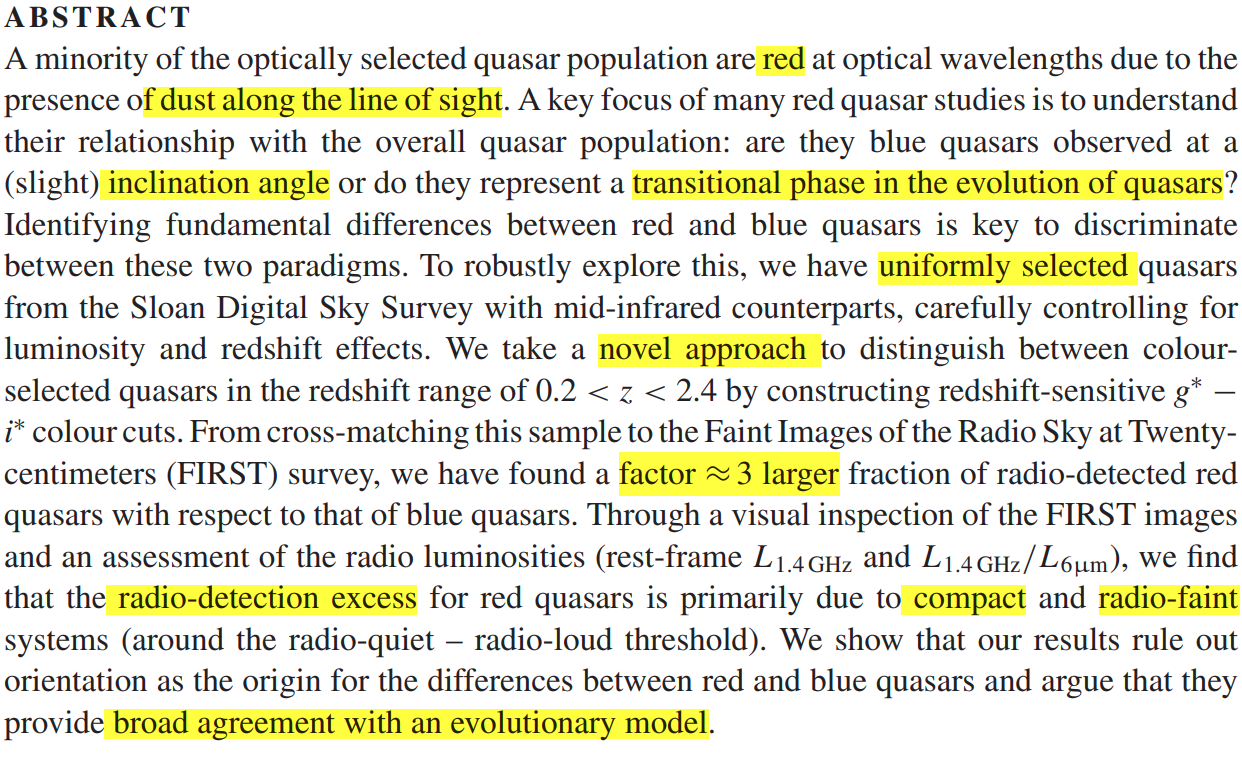
\includegraphics[width=\linewidth]{abstract.png}

}

\section{Introduction}
%\subsection{rQSOs}
\frame{\frametitle{What we know about QSOs:}
\begin{itemize}
\item{Dust in the torus, heated by the accretion disk, emits thermally at MIR: 
5-40 $\mu m$, drops off steeply to FIR 40-500 $\mu m$}
\item{5-10$\%$ of optically detected QSOs are powerful at radio.}
\item{Broad emission lines+power-law continuum: rQSOs with redder continuum challenged this}
\end{itemize}
}
%\subsection{Uncertain nature of rQSOs}
\frame{\frametitle{Uncertain nature of rQSOs }
\begin{enumerate}
\item{Dust reddening of accretion disc emission}

\item{(or) The excess of flux at longer wavelengths: synchrotron or host G contamination?}
\item{(or) Intrinsic red continuum: accretion disk difference and/or Eddingthon ratio
 				difference compared to normal quasars?}
\end{enumerate}
}
\frame{\frametitle{Orientation or Evolution?} 
\begin{itemize}

\item {Difference of nearby obscured/unobscured AGNs: explained by dusty torus viewing angle }
\item {Rare red quasars: Transition between dusty SF and clearing of LOS by outflow/feedback.}
\end{itemize}
}
%\subsection{Challenging rQSOs}
\frame{\frametitle{Challenge in studying rQSOs} 
\begin{itemize}
\item {Broad range of selection approach: optical-NIR-MIR colour criteria, point-source morphologies, and
bright radio emission}
\item {No uniform blue control sample in most studies: z, $M_{BH}$, L, Edd. ratio}
\end{itemize}
}

\section{Samples}
\frame{ \frametitle{Sample selection flowchart}
\centering
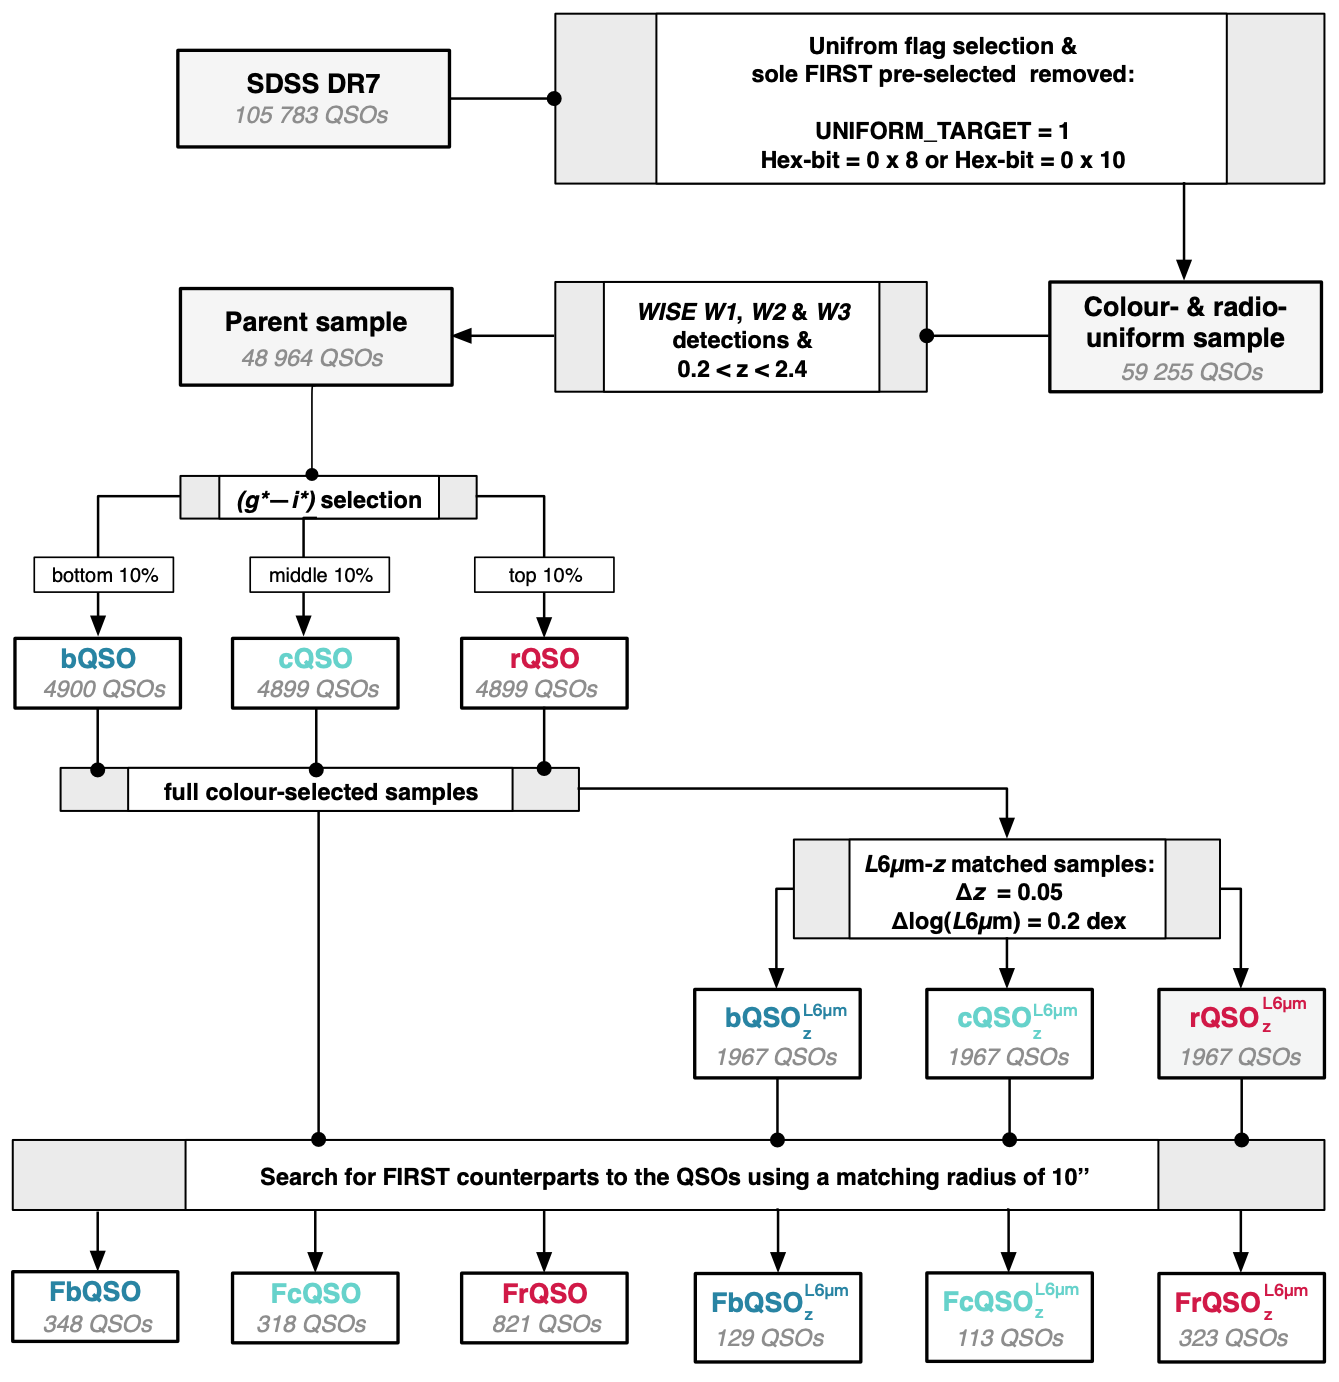
\includegraphics[height=8cm]{figures/flowchart.png}
}

\frame{ \frametitle{Sample statistics} 
\centering
\includegraphics[height=8cm]{t1.png}
}

\frame{\frametitle{Red-shift evolution sensitive sample selection}
\centering
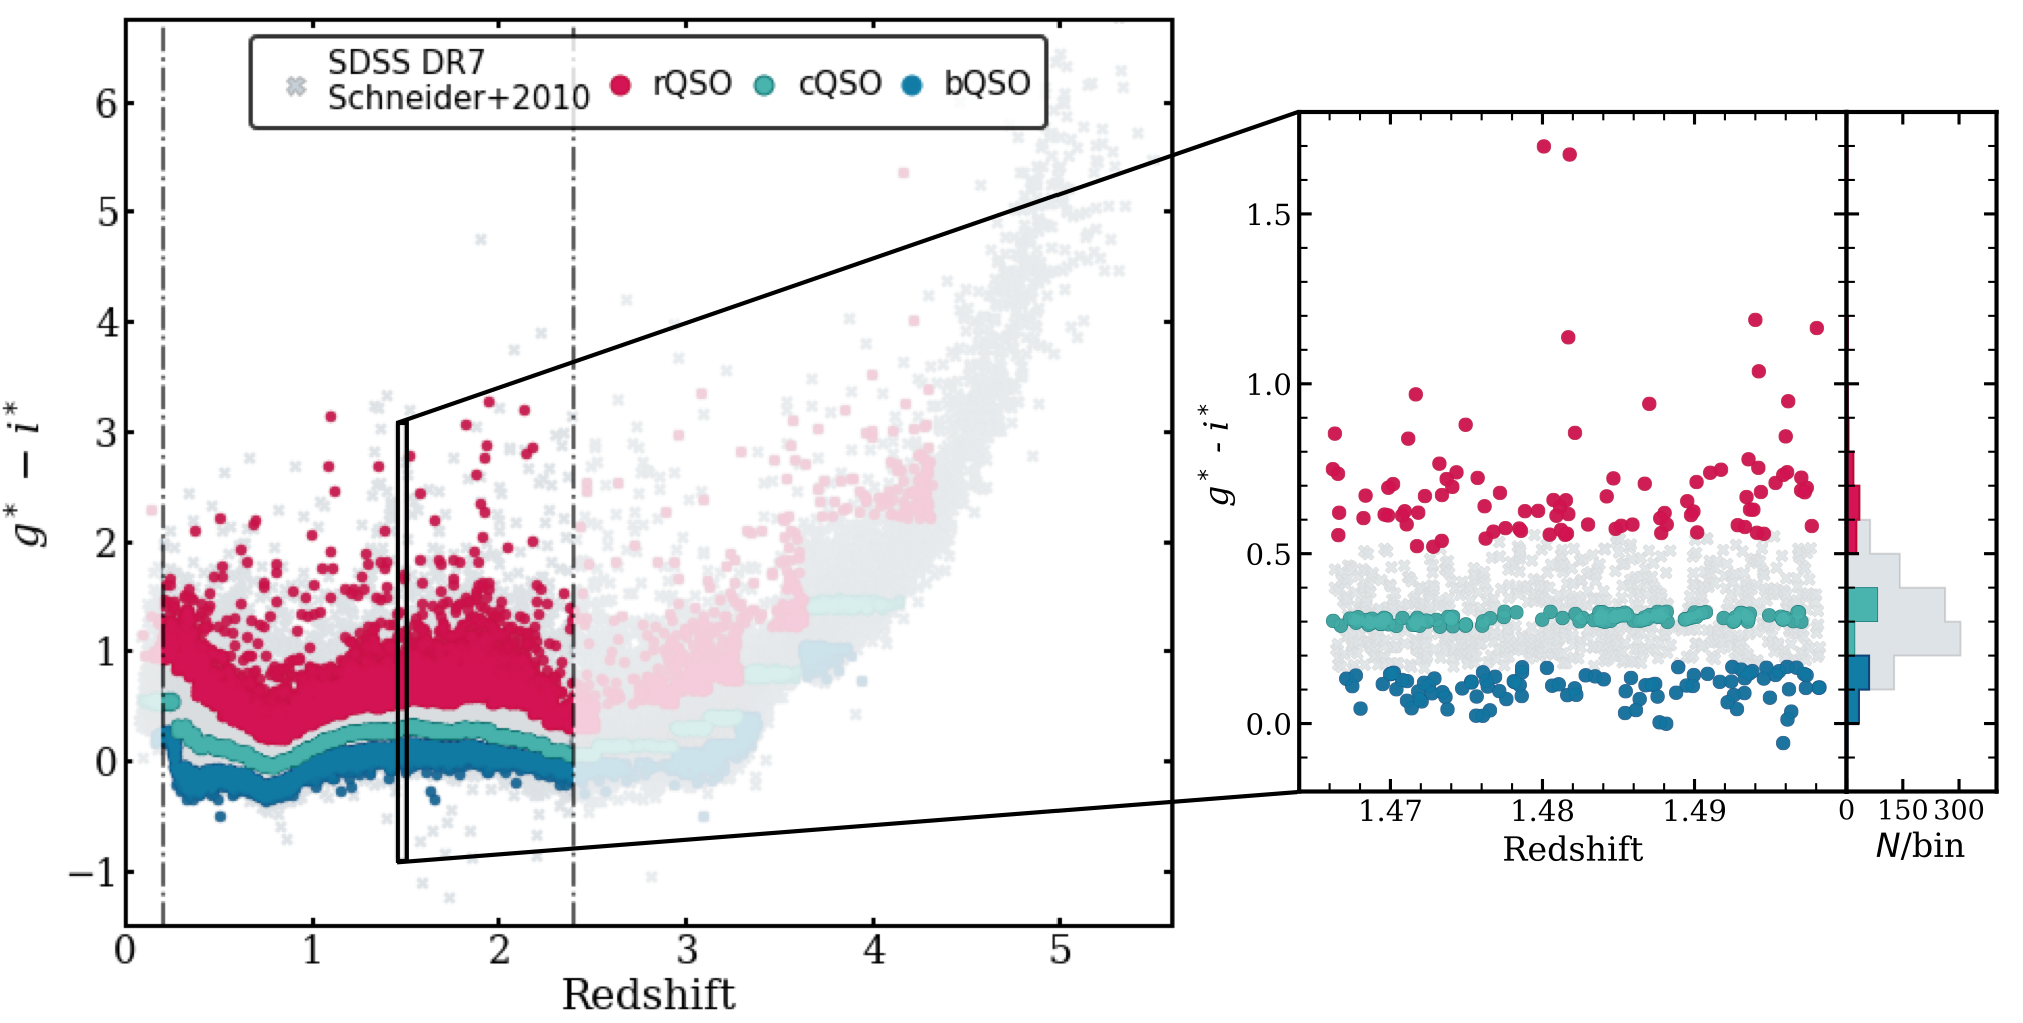
\includegraphics[width=\linewidth]{figures/gi_z.png}
}

\frame{\frametitle{rQSOs are red in both $g^*-i^*$ and $u^*-r^*$ }
\centering
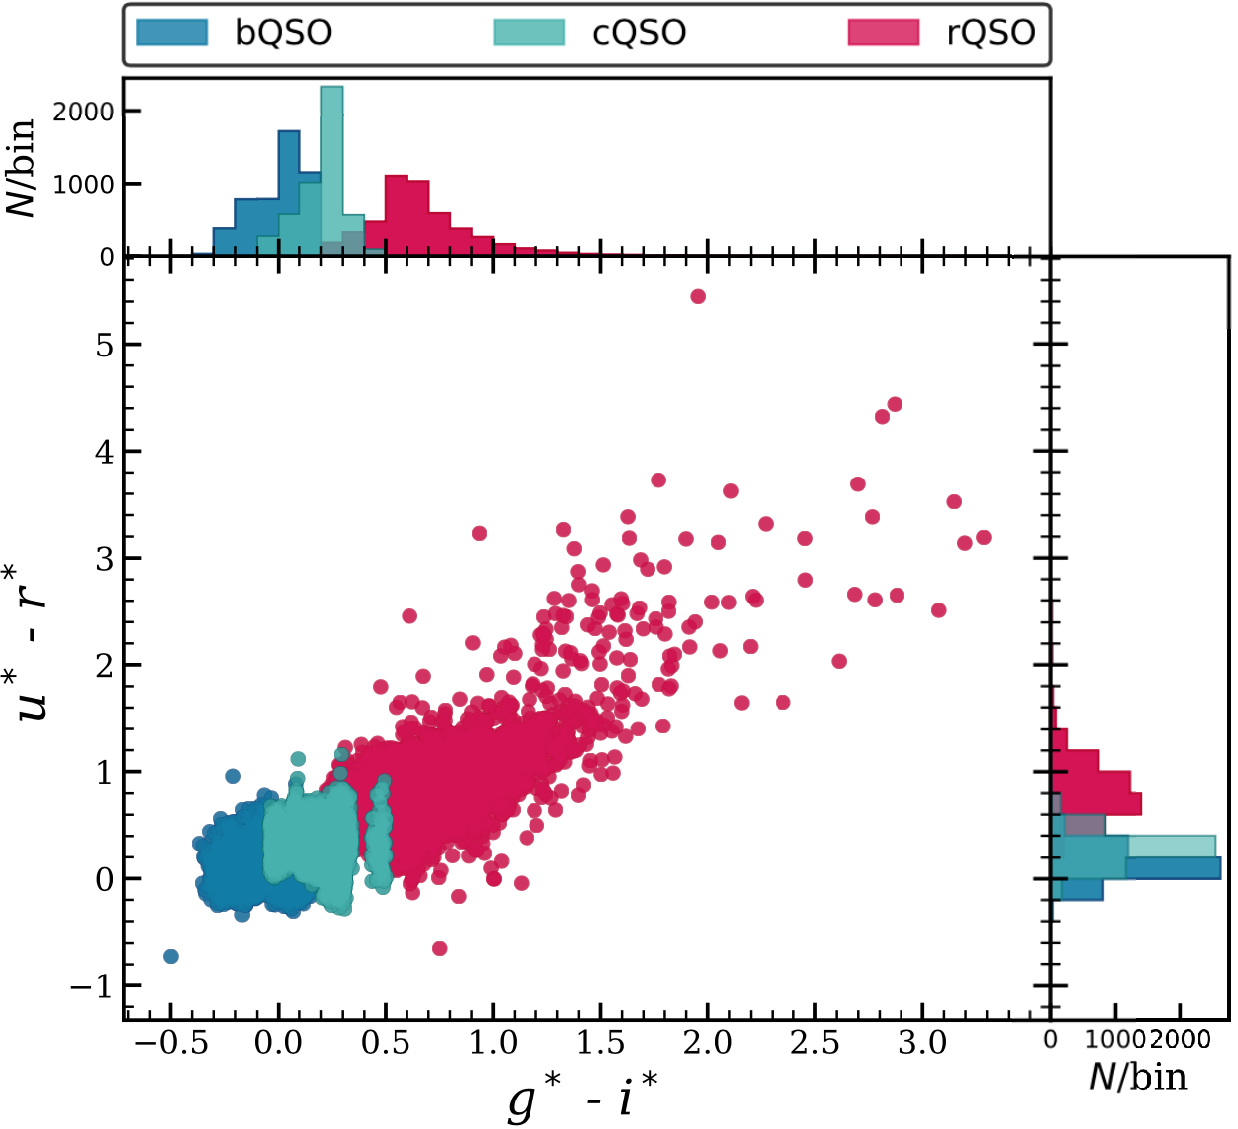
\includegraphics[height=8cm]{figures/sdss_ur_gi_all.png}
}


\frame{\frametitle{Dust-extinction  (SMC, $N_H>2.8\times 10^{28}$  cm$^{-2}$)}
\centering
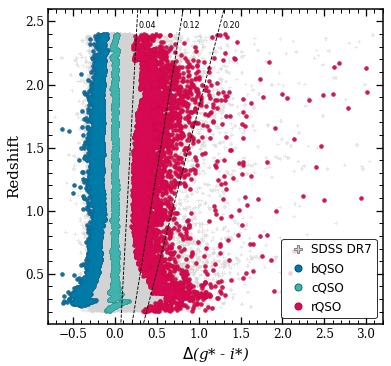
\includegraphics[height=8cm]{figures/delta_GI_extinction.png}}




\frame{\frametitle{AGN Wedge: MIR/FIR $\rightarrow$ AGN/SF}
\centering
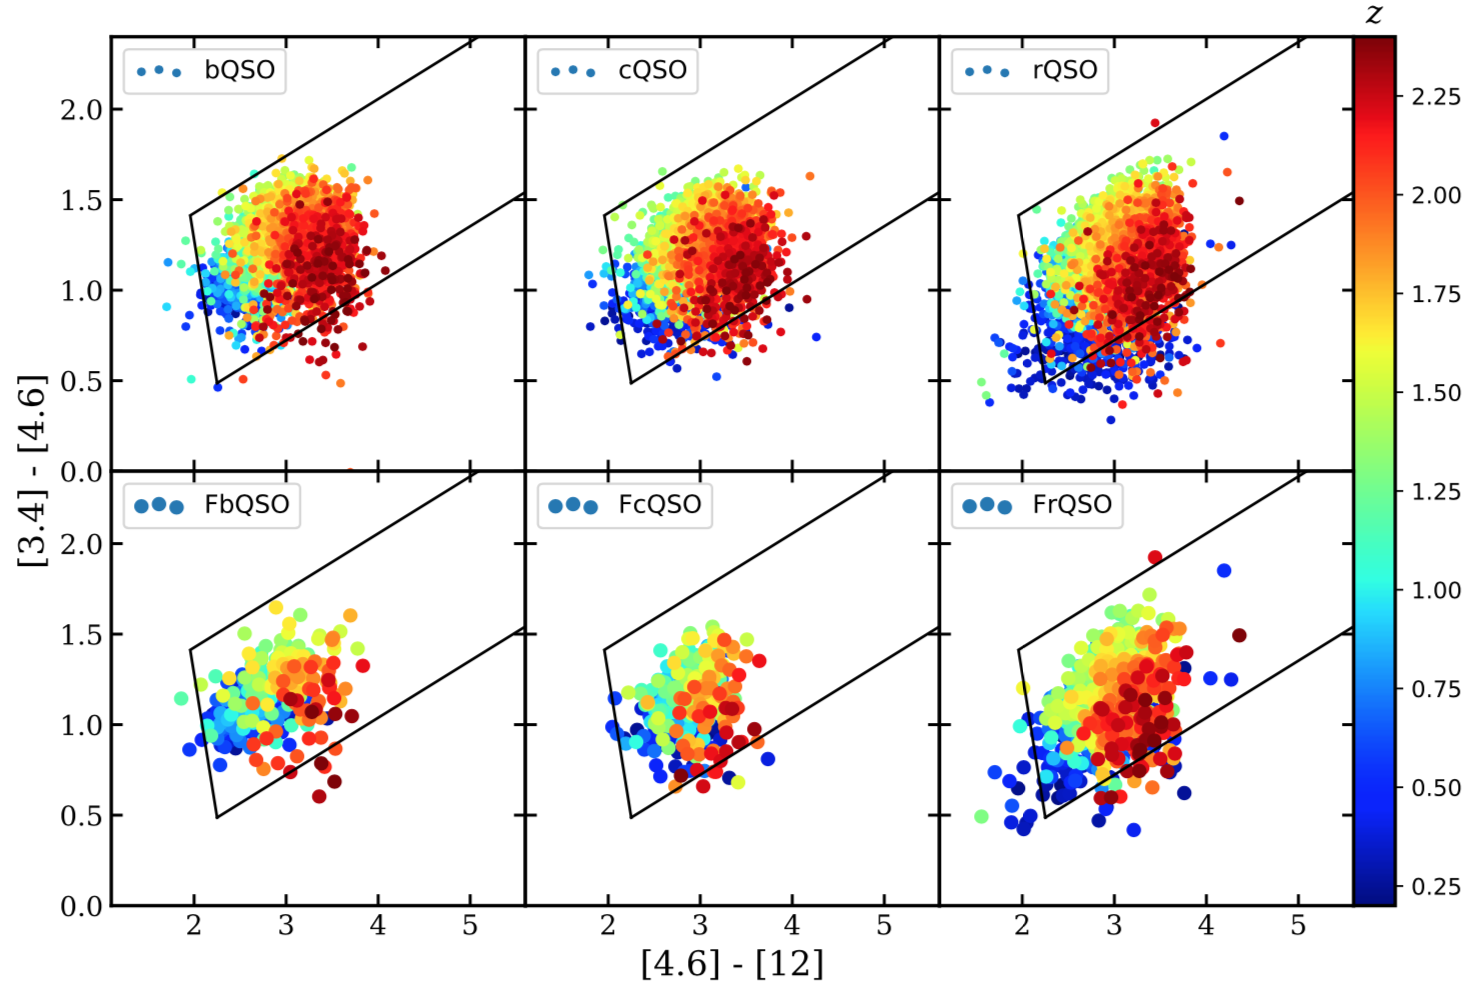
\includegraphics[width=\linewidth]{figures/wise_wedge_combined.png}
}

\frame{\frametitle{Number and percentage outside AGN wedge }
\centering
\includegraphics[width=\linewidth]{t2.png}
}

\frame{\frametitle{Lum$_{6 \mu m}$ vs. z}
\centering
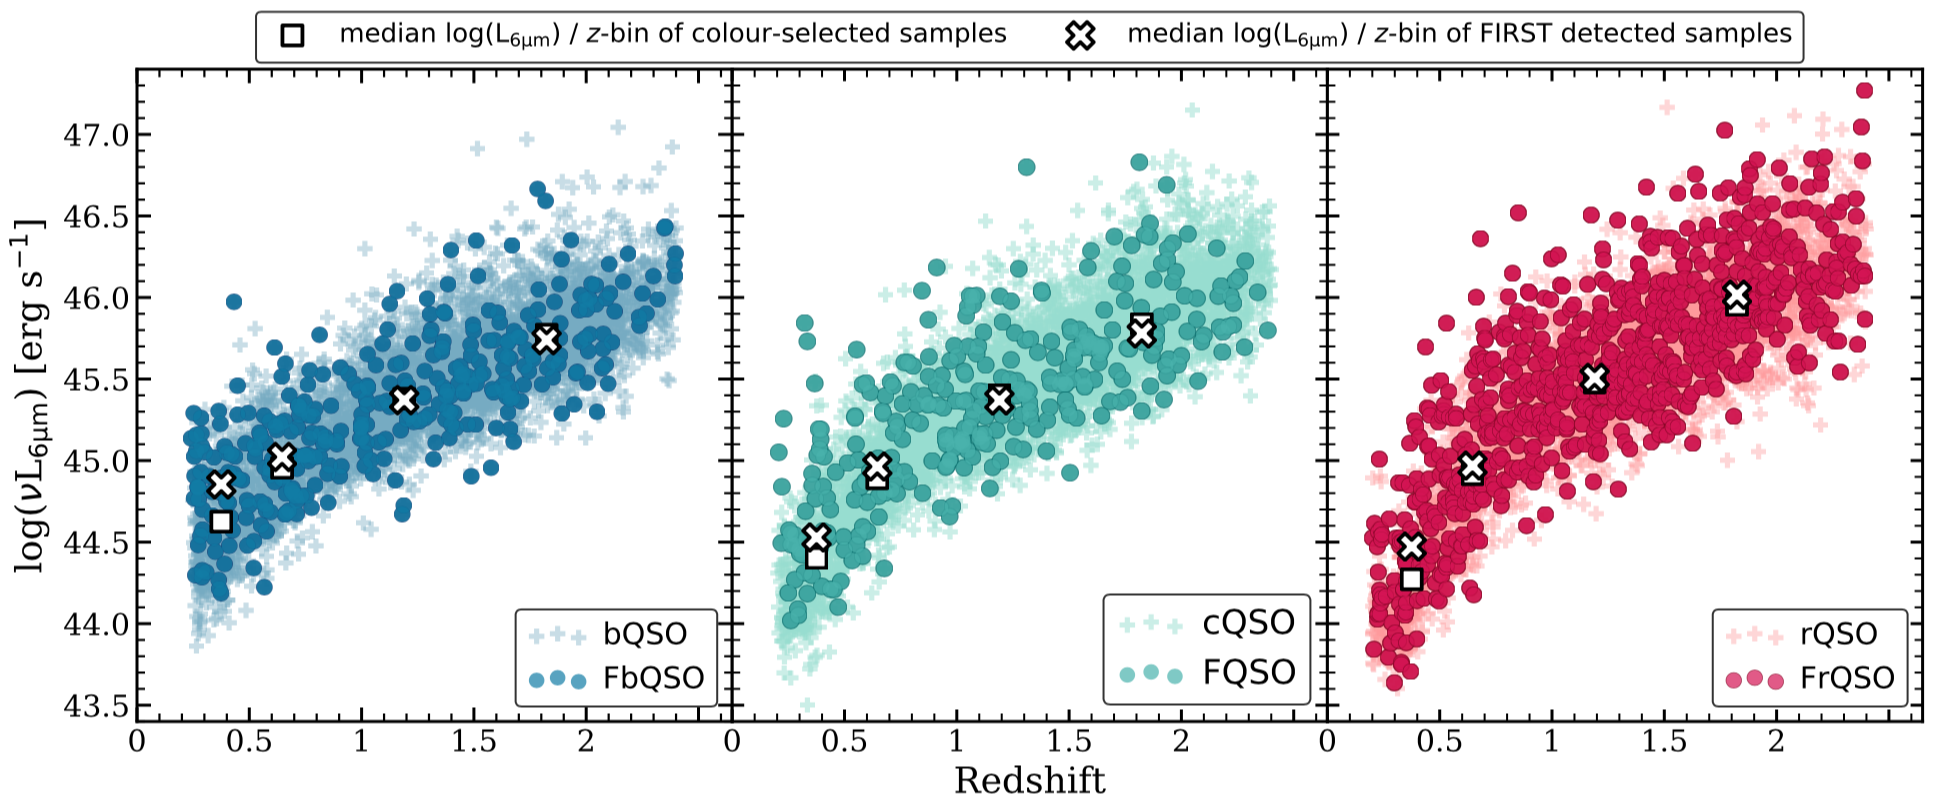
\includegraphics[width=\linewidth]{figures/logL6um_z.png}
}

\section{Radio Luminosity}
\frame{\frametitle{Luminosity distribution}
\centering
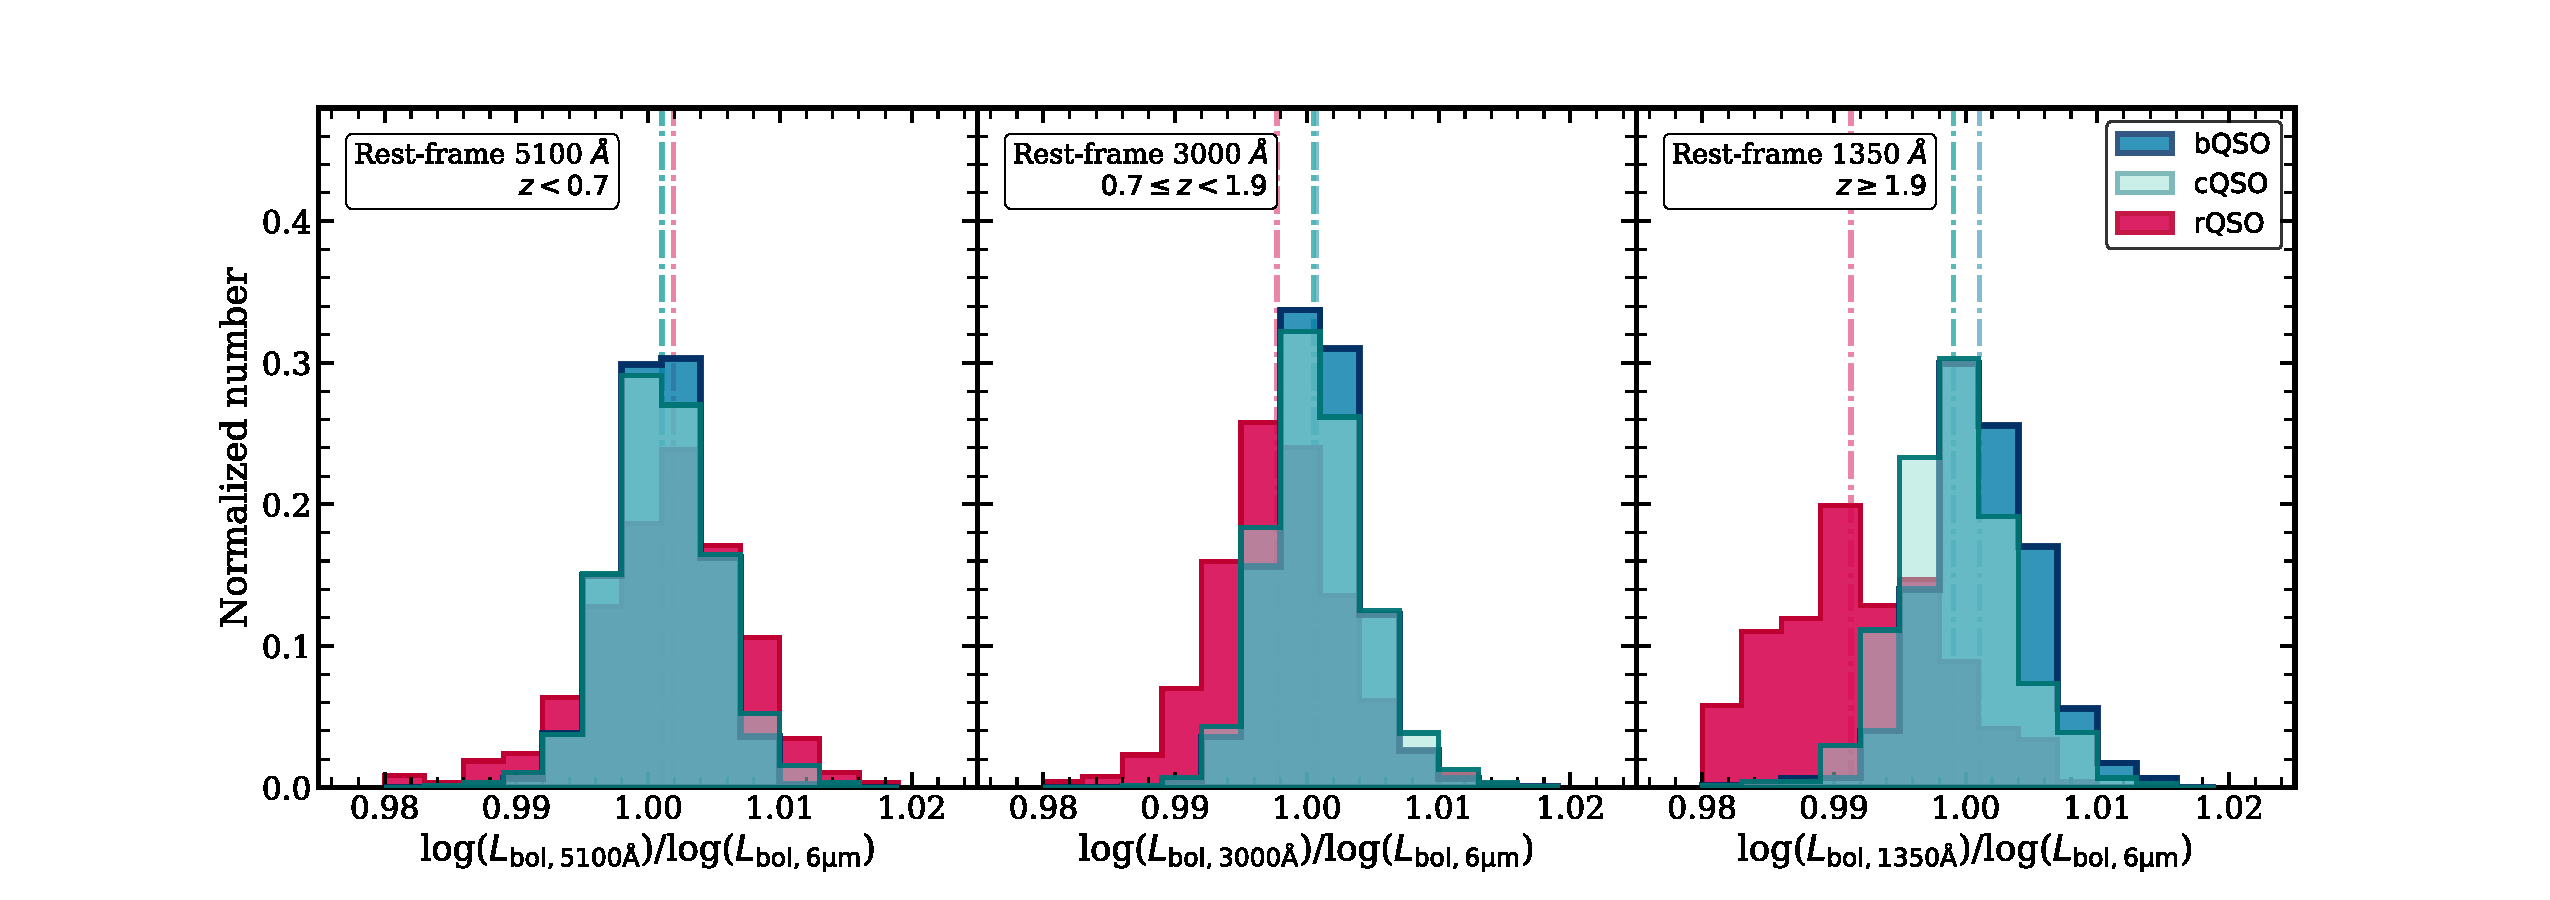
\includegraphics[width=\linewidth]{figures/L6mu_vs_Lbol_hist_lines}
}
\section{Radio Detection}
\frame{\frametitle{Radio detection}
\centering
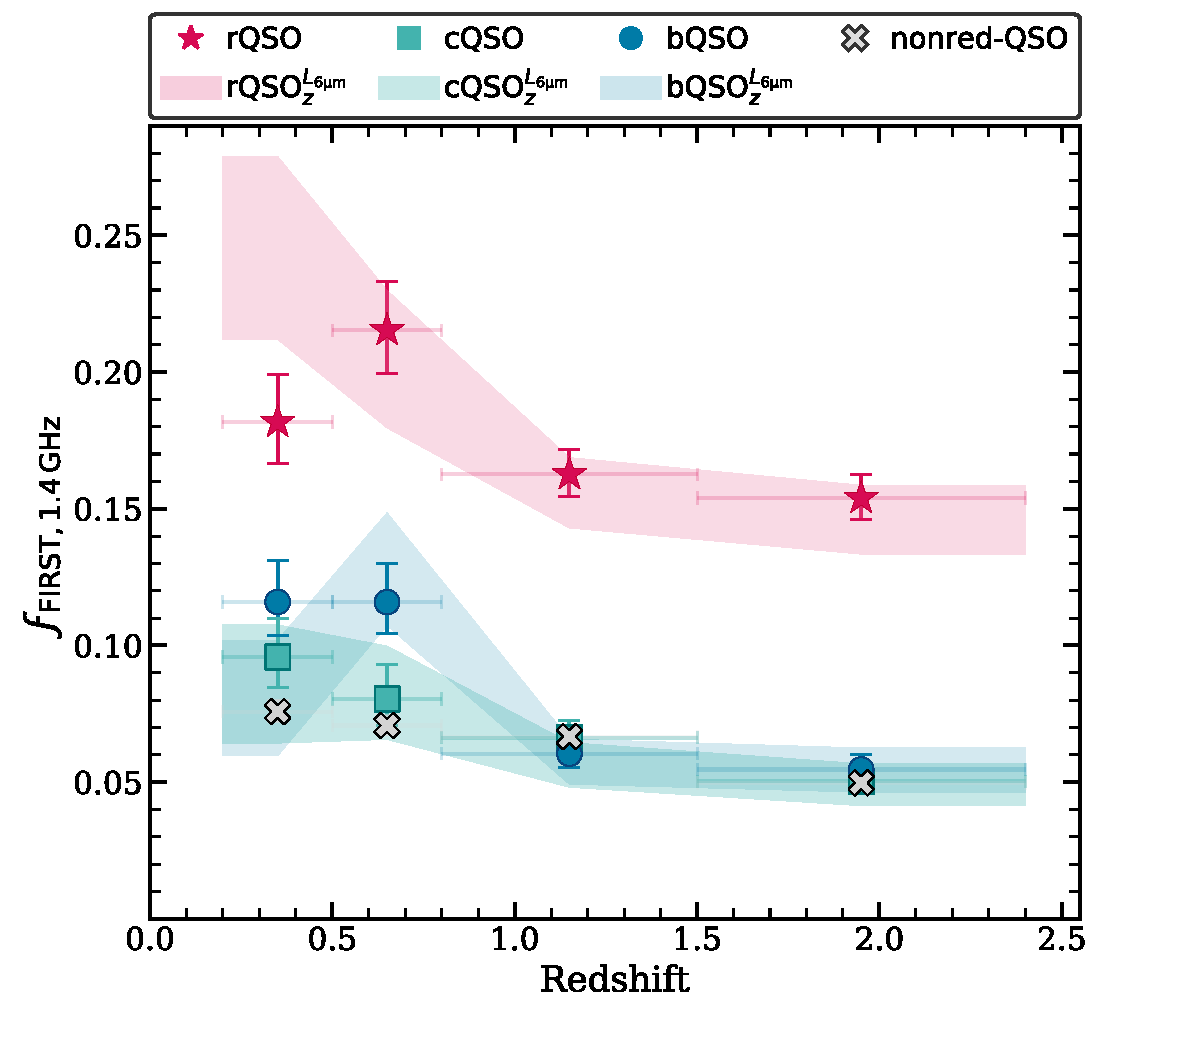
\includegraphics[height=8cm]{figures/radio_detection_frac}
}


\frame{\frametitle{FIRST detection percentage}
\centering
\includegraphics[width=\linewidth]{t3}
}


\frame{\frametitle{FIRST radio detection in i-g quantiles }
\centering
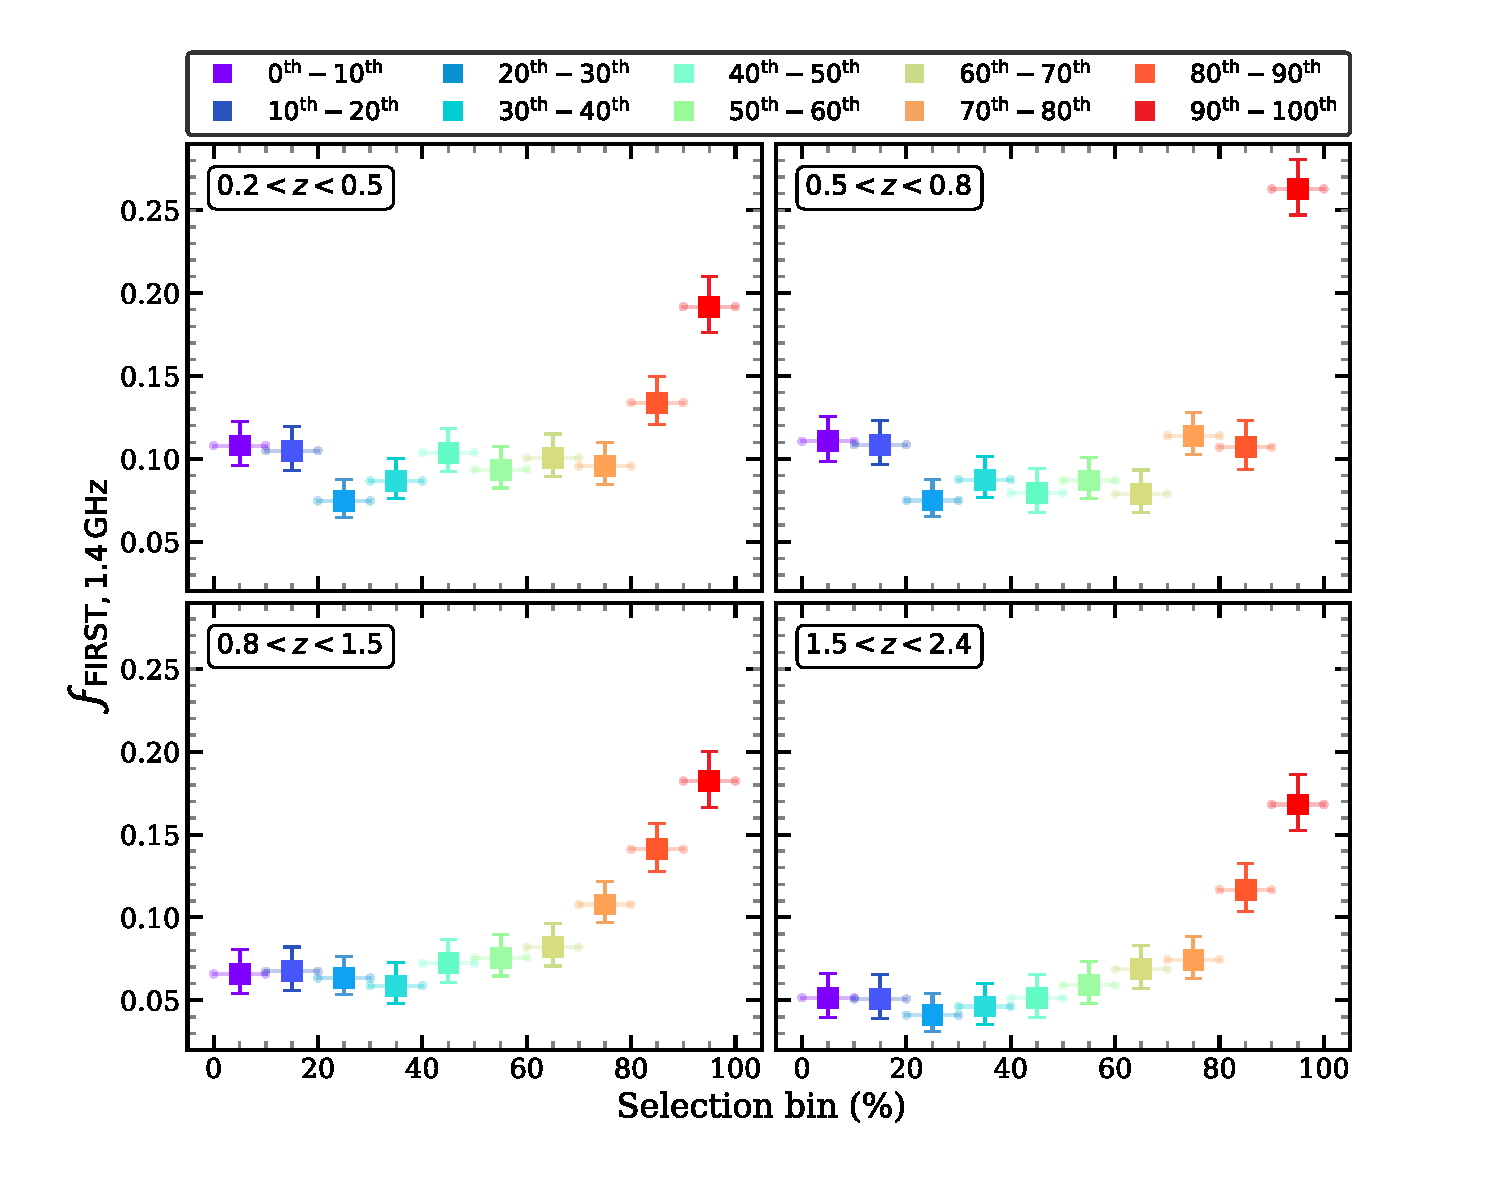
\includegraphics[width=\linewidth]{figures/radiodetection_frac_10per.pdf}
}

\section{Radio Morphology}
\frame{\frametitle{Radio morphology Classificaion}
\centering
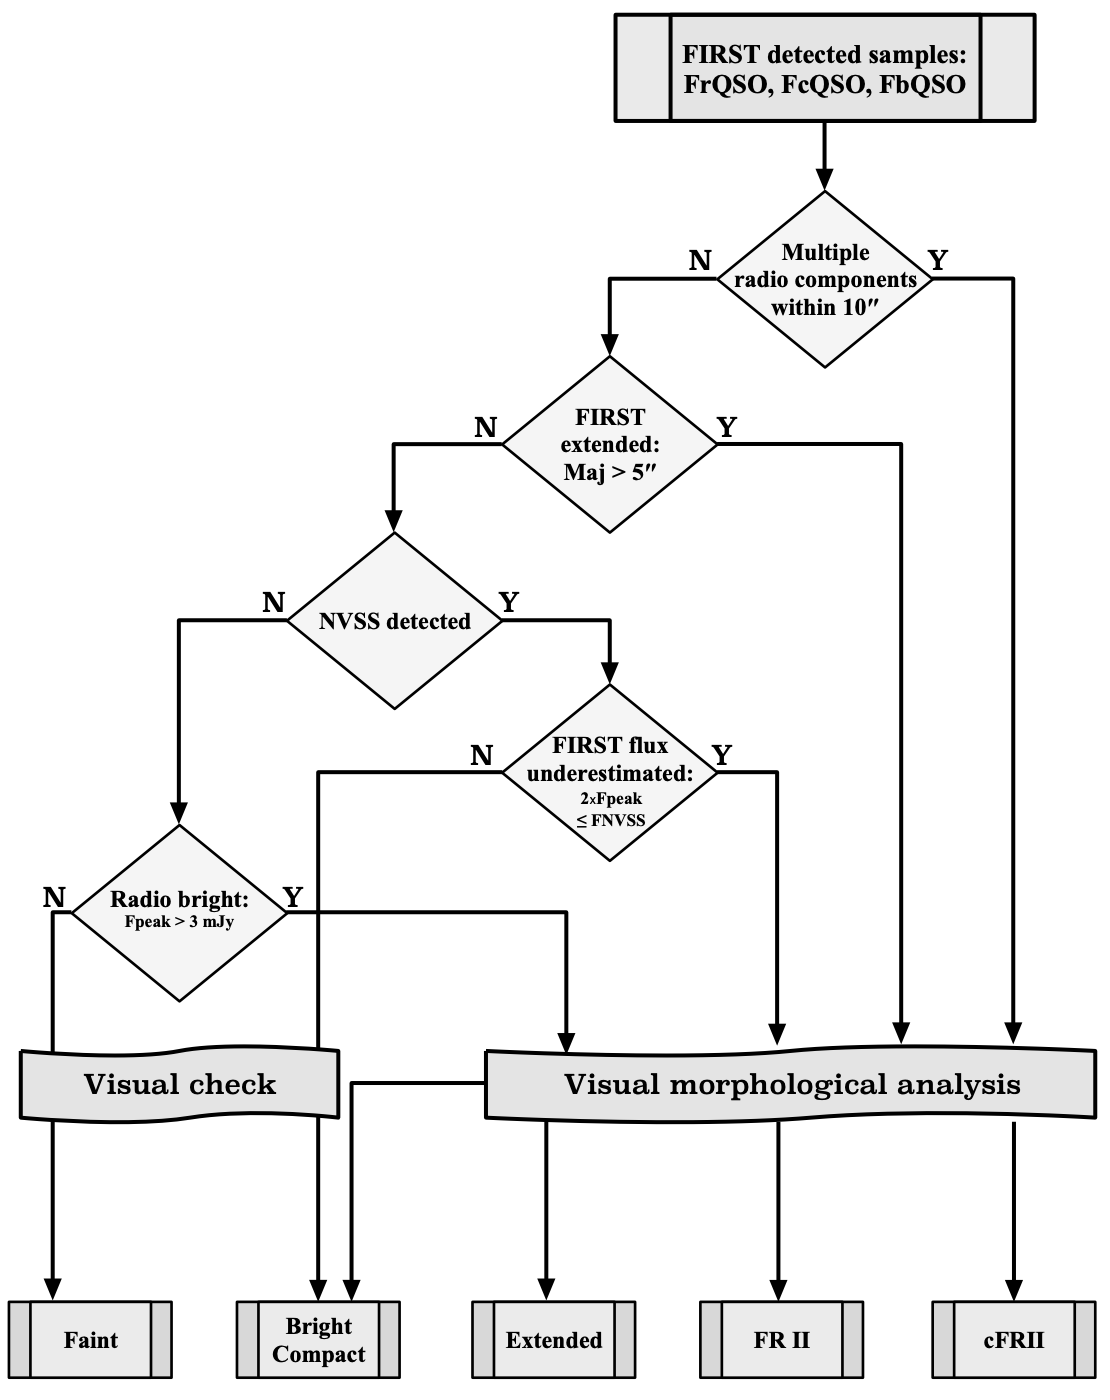
\includegraphics[height=8cm]{figures/FIRST_flowchart}
}

\frame{\frametitle{Radio Morphology Classes}
\centering
\includegraphics[width=\linewidth]{t4}
}


\frame{\frametitle{NVSS vs. FIRST flux at 1.4 GH}
\centering
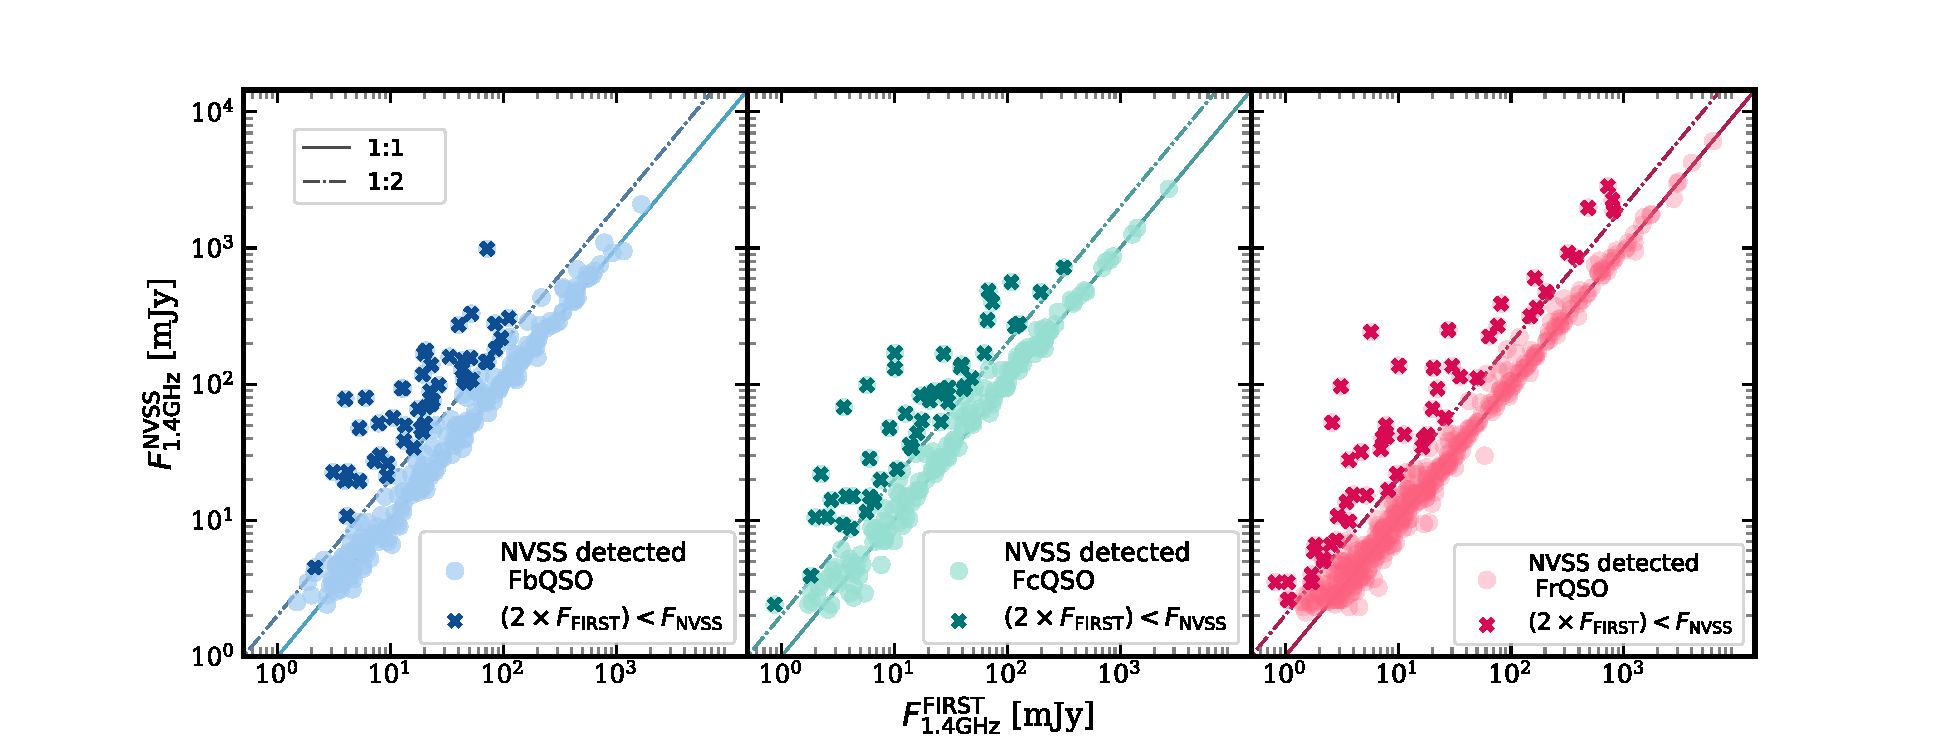
\includegraphics[width=\linewidth]{figures/FIRST_summed_fluxes}
}


\frame{\frametitle{Radio Morphology and Color}
\centering
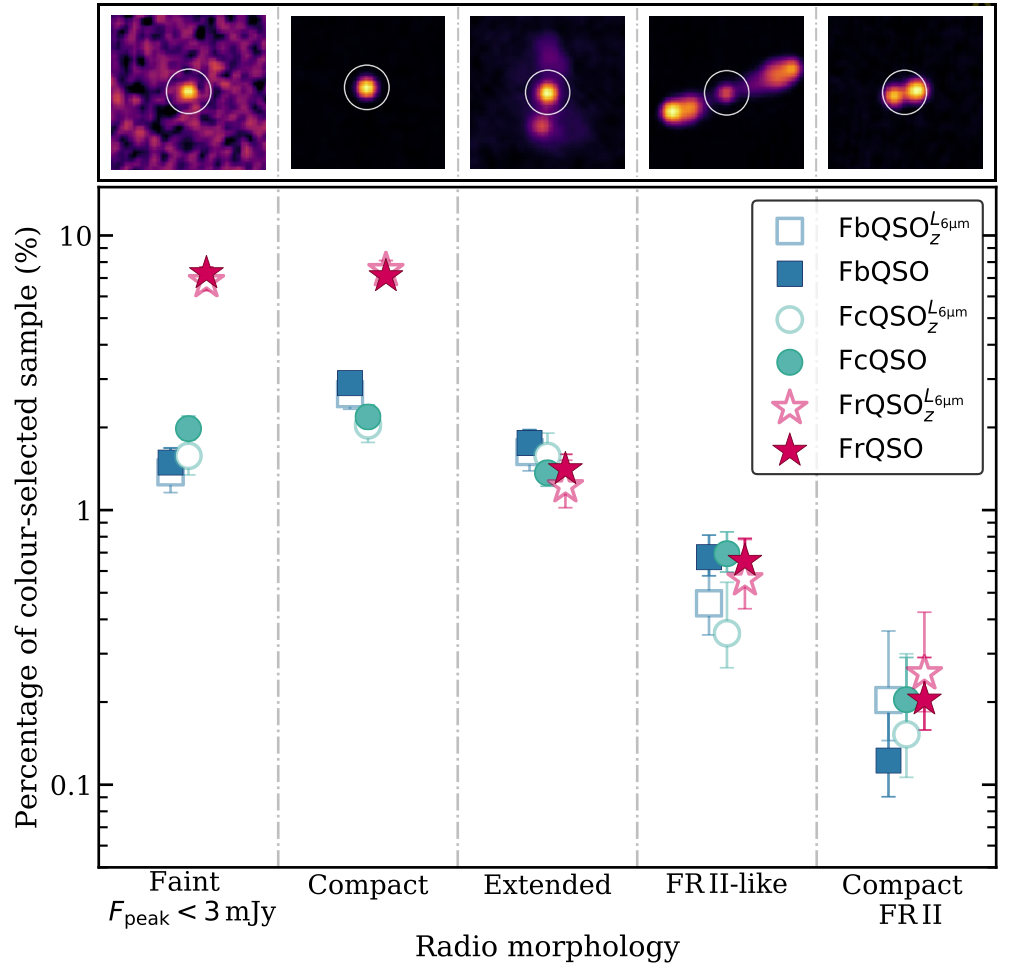
\includegraphics[height=8cm]{figures/FIRST_morphology_fractions}
}



\frame{\frametitle{Quasars in each morphology classes}
\centering
\includegraphics[height=7cm]{t5}
}


\frame{\frametitle{Radio loudness of FbQSOs, FcQSOs, and FrQSOs}
\centering
\includegraphics[height=5cm]{t6}
}


\frame{\frametitle{Radio luminosity at 1.4 GHz vs. z for FbQSO,FcQSO,and FrQSO}
\centering
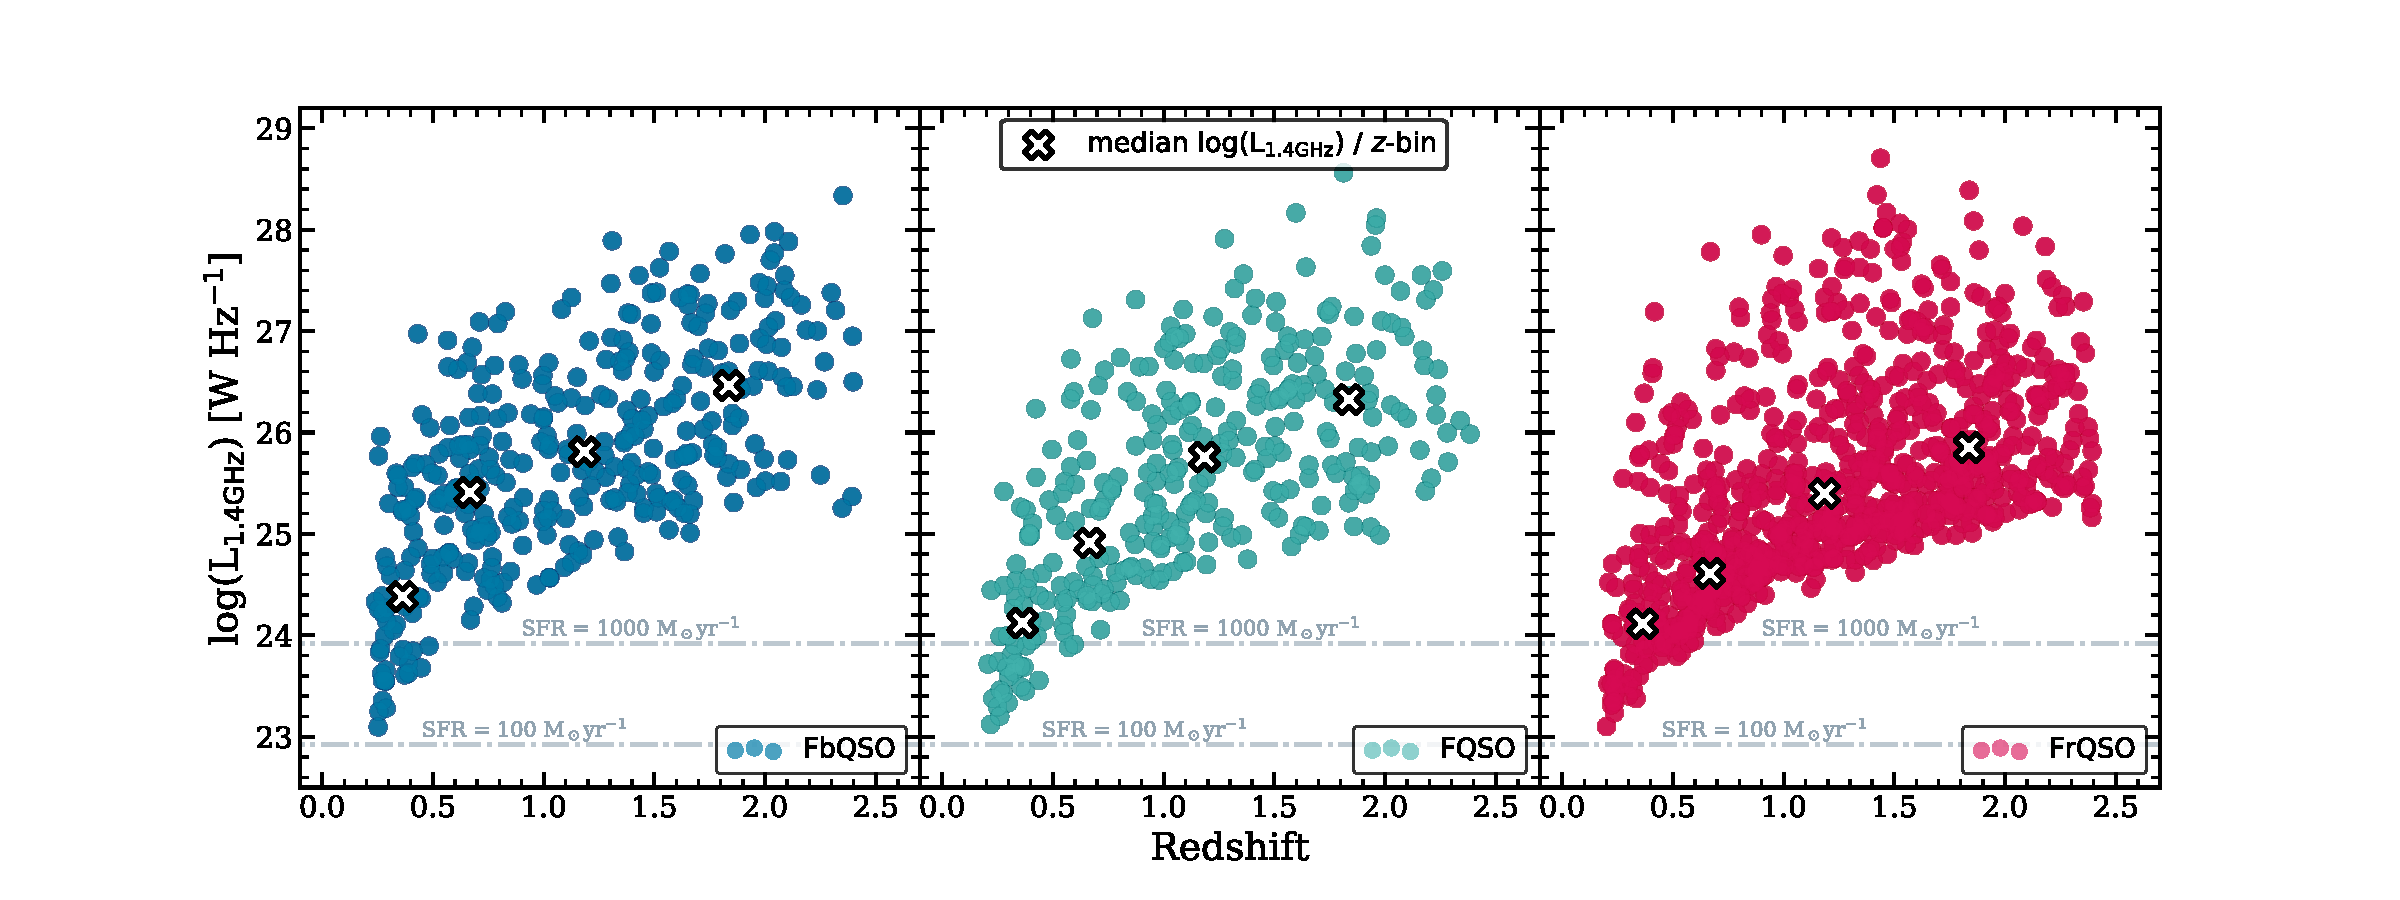
\includegraphics[width=\linewidth]{figures/Lradio_vs_z_summed_fluxes}
}

\frame{\frametitle{Relative fraction of FIRST-detected BALQSOs compared
to FcQSOs as a function of R}
\centering
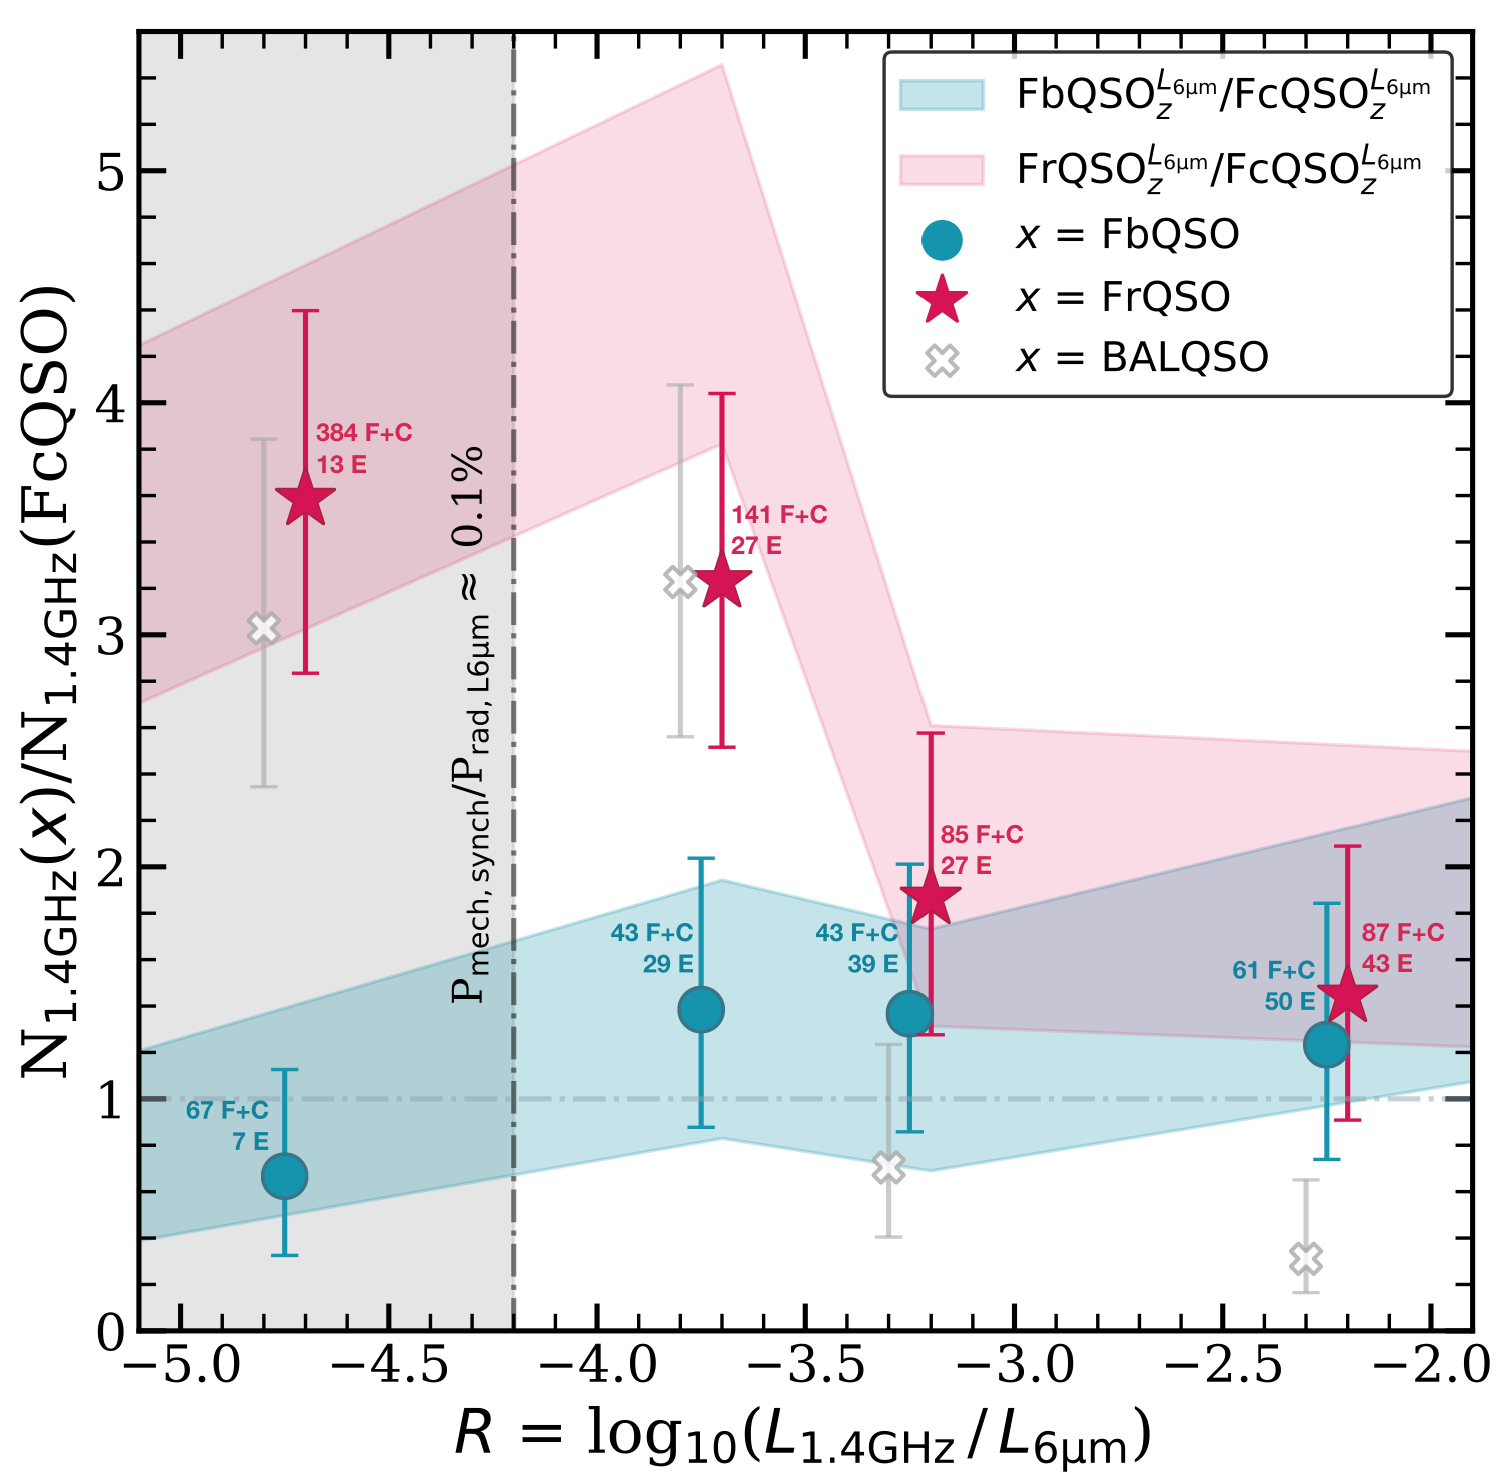
\includegraphics[height=7cm]{figures/radio_detection_frac_radioloudness}
}


\frame{\frametitle{Estimated bolometric luminosity
(Lbol, 6$\mu m$) vs. FWHM for the b,c,rQSO$^{L_{6\mu m}}_z$
}
\centering
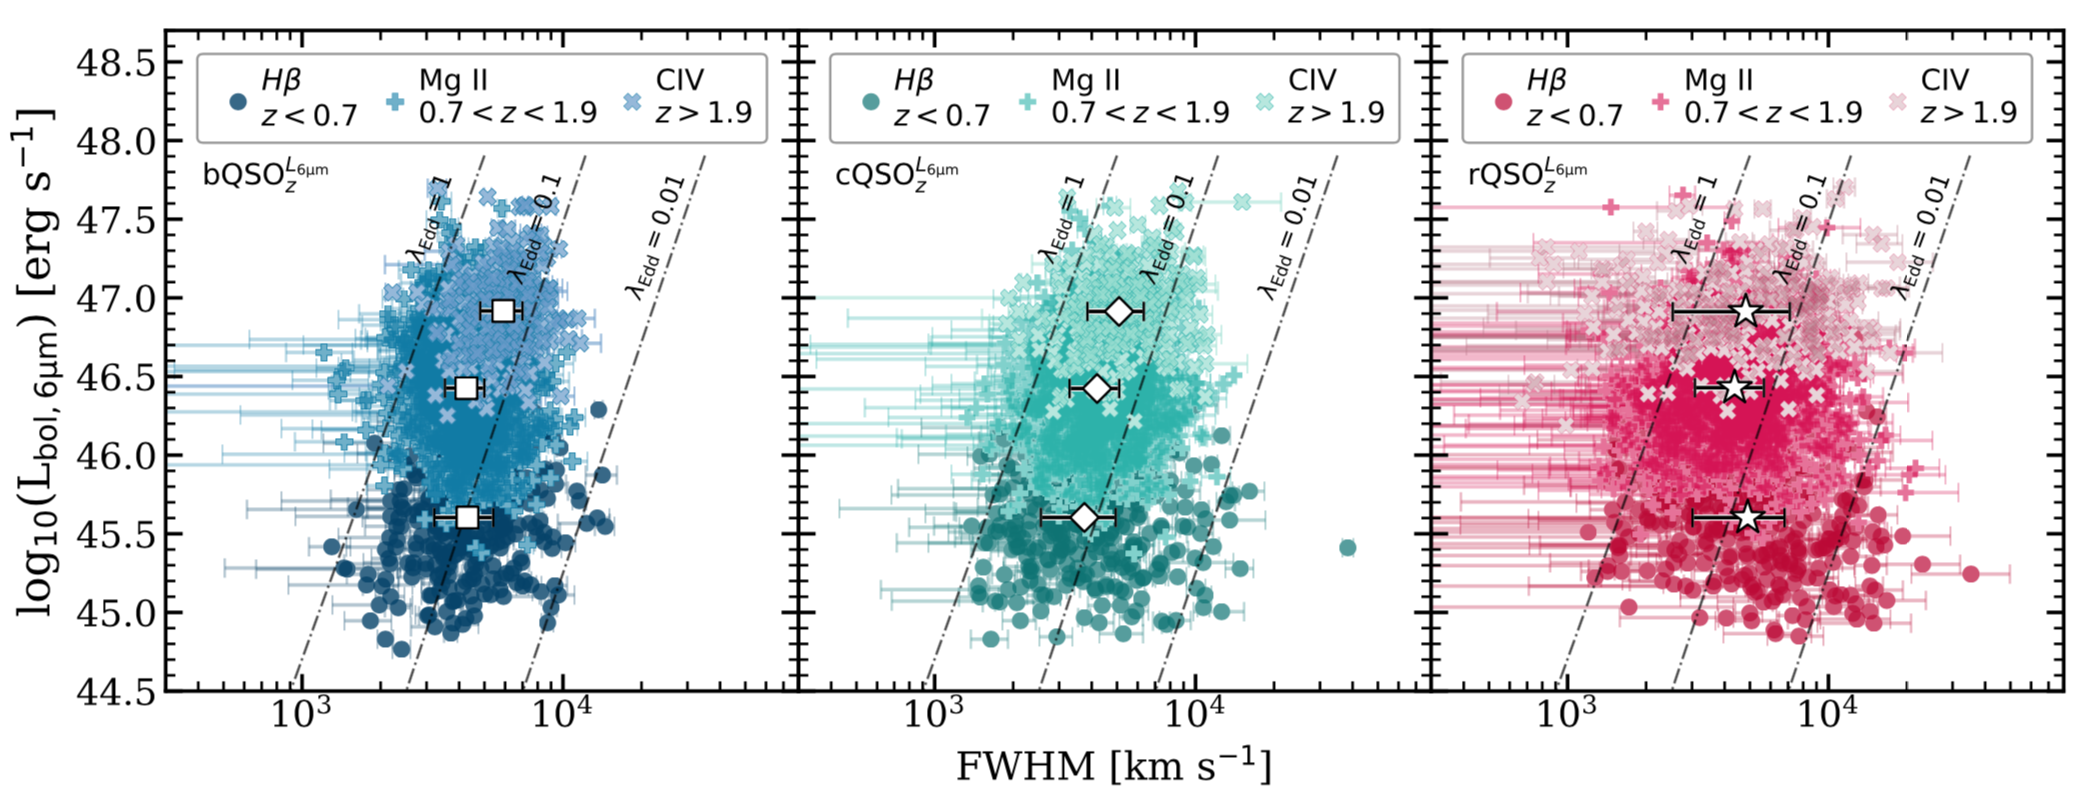
\includegraphics[width=\linewidth]{figures/fwhm_L6um.png}
}

\section{Orientation or evolution?}  


\end{document}












































